\documentclass[10pt,a4paper]{article}
\usepackage[a4paper,margin=1.8cm]{geometry}
\usepackage[T1]{fontenc}
\usepackage{lmodern,microtype}
\usepackage{amsmath,amssymb}
\usepackage{graphicx,booktabs,caption,subcaption}
\usepackage[hidelinks]{hyperref}
\usepackage{enumitem}
\setlist{nosep,leftmargin=*}
\captionsetup{font=small,labelfont=bf}
\setlength{\parskip}{3pt}\setlength{\parindent}{0pt}
\newcommand{\repo}{https://github.com/ijsukhmani13-star/eep55c36-bit-loading}

\title{\vspace{-1.2cm}\textbf{Discrete Bit Loading for DMT: Linear Scan versus Priority Queue}\\
\large EEP55C36 Computational Methods and Algorithms --- Final Project, Track D}
\author{Inderjeet Singh Sukhmani}
\date{November 2026}

\begin{document}
\maketitle
\vspace{-0.8cm}

\section{Problem and paper}
\emph{Discrete multitone} (DMT) modulation splits a wired channel (e.g.\ DSL) into $N$
narrow subchannels called \emph{tones}. Tones with a strong channel and little noise can carry
more bits. \emph{Bit loading} decides how many bits, and therefore how much transmit energy, each
tone gets, under a total energy budget. Campello~\cite{campello} gives a practical
framework for this integer problem. \textbf{Reproduction scope:} I implement only its
\emph{discrete marginal-energy (greedy) allocation core} with a per-tone cap, starting from zero
bits. The paper's initialisation and acceleration steps are not reproduced. All data are
\textbf{synthetic} (Sec.~4). No physical bit-error performance is claimed.

\section{Mathematics and implementation}
For tone $i\in\{0,\dots,N-1\}$ the received symbol is $y_i=h_ix_i+n_i$ with complex channel gain
$h_i$ and zero-mean noise of variance $\sigma_i^2>0$. With transmitted energy $e_i=\mathbb{E}|x_i|^2$
(normalised units), the received SNR is $g_ie_i$, where $g_i=|h_i|^2/\sigma_i^2$ is the
channel-to-noise ratio per unit energy. Under the standard \emph{gap approximation} with gap
$\Gamma\ge1$, a tone carrying $b_i$ bits needs energy
\begin{equation}
e_i(b_i)=\frac{\Gamma}{g_i}\bigl(2^{b_i}-1\bigr),\qquad
\max_{\mathbf b}\sum_i b_i\ \ \text{s.t.}\ \ \sum_i e_i(b_i)\le E_{\max},\ \ b_i\in\{0,1,\dots,b_{\max}\}.
\end{equation}
The \emph{optimisation objective} is total bits, $B=\sum_ib_i$. This is not the same as engineering task quality: a
predicted rate is reliable only if $g$ and $\Gamma$ are right.
The marginal cost of one more bit on tone $i$ is
$\Delta_i(b_i)=e_i(b_i{+}1)-e_i(b_i)=(\Gamma/g_i)\,2^{b_i}$, so it doubles after every bit.
\textbf{Greedy rule:} start from $\mathbf b=\mathbf 0$. Repeatedly take the eligible tone ($b_i<b_{\max}$)
with the smallest $\Delta_i$. Stop when that cost exceeds the remaining energy. Ties go to the
smallest index. Each tone's costs increase, and a later bit requires the cheaper earlier ones. So
choosing the globally cheapest increments gives, for every bit count, the cheapest feasible set.
Once the cheapest increment is unaffordable, no allocation with one more bit fits. The rule is
therefore optimal \emph{for this separable model}. The argument fails if tones are coupled (e.g.\
crosstalk), if bit steps are unequal, or if the objective changes. This is the main assumption, and it is
violated in multi-user DSL with crosstalk.

\textbf{Baseline} (\texttt{src/baseline.py}, \texttt{allocate\_scan}): masks capped tones with
\texttt{np.where} and selects with \texttt{np.argmin}, which returns the first index on ties. This is
$\Theta(N)$ per increment and $\Theta(NB)$ in total. The safeguards are input validation ($g_i>0$, finite budget,
integer cap), an empty-input path, and \texttt{inf} for capped tones, which also stops the loop once every tone is full.
\textbf{Verification} (\texttt{tests/}, 348 checks, \texttt{python -m pytest}):
\begin{itemize}
\item \emph{Hand-computed cases.} $g=[1,1]$, $\Gamma=1$ gives $[1,1]$ at $E_{\max}=3$ and $[2,1]$ at $E_{\max}=4$.
  The course guide quotes $[2,1]$ ``using energy 3'' at $E_{\max}=3$, but $e(2)+e(1)=4>3$, so that allocation is
  infeasible under the stated model. Exhaustive search agrees with my value.
\item \emph{Limits.} Zero budget, a budget below the cheapest bit, $b_{\max}=0$, saturation at the cap, and empty input all behave correctly.
  Invalid inputs raise \texttt{ValueError}.
\item \emph{Optimality.} On 40 random tiny cases ($N\le3$, $b_{\max}\le3$), $B$ equals the exhaustive-search
  optimum, with the minimum energy for that $B$.
\item \emph{Properties.} Energy used $\le E_{\max}$ and matches the closed form. Outputs are finite, with
  shape $(N,)$ and integer type. $B$ never decreases with the budget, a stronger tone never gets fewer bits,
  and the input is never mutated.
\end{itemize}
These checks establish \emph{code correctness} for the model. They say nothing about whether the model
describes a real line (Sec.~5).

\section{The change: priority-queue selection}
\textbf{Exactly what changes} (\texttt{src/modified.py}): only the \emph{selection step}. The next-bit
costs are kept in a binary min-heap of $(\Delta_i,i)$ pairs (Python \texttt{heapq}). The cheapest
increment is read from the top in $O(1)$. After a purchase, that entry is replaced by $(2\Delta_i,i)$ and
sifted down in $O(\log N)$. A tone reaching $b_{\max}$ is popped. Tuple ordering gives the same
first-index tie rule. The energy model, the stopping rule and the order of floating-point operations
are unchanged, and doubling is exact in binary. The output is therefore expected to be
\emph{bit-for-bit identical}, and only the cost changes: $O(N)$ setup (\texttt{heapify}) plus $O(B\log N)$,
compared with $\Theta(NB)$. Priority queues for repeated minimum selection are standard~\cite{clrs}, and the course
guide lists this change for the track. The implementation is my own. Setup
(\texttt{heap\_setup}) and allocation (\texttt{heap\_allocate}) are separate functions so that they can be timed separately.

\textbf{Hypothesis:} identical allocations, with a speed advantage that grows with $N$.
\textbf{Predicted to help} when there are many tones and many increments. \textbf{Predicted to hurt} with tiny
budgets, where the $O(N)$ heap build is not repaid. A further risk is that the baseline's
\texttt{argmin} is vectorised C code, while the heap runs in interpreted Python.
\textbf{Ablation:} \texttt{selector="list-scan"} keeps every other decision of the modified code (Python
lists, same loop, same arithmetic) and switches off only the heap, using a linear Python scan instead.
This separates the data-structure effect from the NumPy-versus-Python effect.

\section{Experiments}
\textbf{Data.} The synthetic 8-tap multipath channel from the course guide uses tap powers $\propto e^{-\ell/2}$, normalised to 1,
$\sigma^2=0.1$, and $h=\mathrm{FFT}_N(\text{taps})$ (\texttt{src/data.py}). There are two information conditions, given
identically to both methods: \emph{true} $g$ (ideal), and \emph{calibrated} $\hat g$ from 20 averaged unit pilots and
20 noise-only observations. The fixed model settings are $\Gamma=9.8$\,dB (uncoded QAM, symbol-error rate $\approx10^{-7}$)
and $b_{\max}=15$.
\textbf{Separation.} Seeds 0--19 (development) were used for debugging and the tests. Seeds 100--119 (validation) were used to select the
energy per tone $\rho$ in $E_{\max}=\rho N$, by the rule ``mean bits/tone closest to 5'' (mid-range, so neither
budget-starved nor cap-saturated). This gave $\rho=40$ (4.80 bits/tone). Seeds 1000--1029 (test) are used only for reported
results. No supervised training is needed. Each case is an independent channel realisation.
\textbf{Protocol.} The main experiment uses $N\in\{64,256,1024\}\times\{$true, calibrated$\}\times30$ paired cases. The stress cases are:
(i)~a budget sweep $\rho\in[0.01,40]$ at $N=1024$; (ii)~$\hat g$ from 4/20/100 pilots, with the resulting allocation's
energy evaluated on the true $g$; and (iii)~a perfectly flat channel, where every selection is a tie. A scaling run up to $N=4096$ is
also included.
\textbf{Metrics.} The \emph{primary metric}, fixed in advance, is the paired speed-up $t_{\text{scan}}/t_{\text{heap}}$ per case
(larger is better), summarised as a geometric mean with a 95\% $t$-interval on the log ratios over independent channel
realisations. The secondary metrics are exact allocation agreement, $B$, energy and true-budget overspend.
\textbf{Timing.} Each measurement uses \texttt{time.perf\_counter} with the garbage collector off, 1 warm-up run and the median of 5 repeats. Heap
setup is included in the heap time and also reported separately. The machine is an Intel Xeon @ 2.1\,GHz (2 vCPU) running Ubuntu 24.04,
with Python 3.13.18 and NumPy 2.5.3. Runtimes will differ on other machines, but allocations should not.

\section{Results and interpretation}
\begin{table}[h]\centering\small
\caption{Main comparison, true $g$, $\rho=40$, 30 paired test cases per row. Median times include setup.
Intervals are 95\% CIs of the geometric mean. The calibrated-$\hat g$ rows give similar speed-ups (6.5--7.1$\times$).}
\label{tab:main}
\begin{tabular}{rrrrrrc}\toprule
$N$ & mean $B$ & scan (ms) & heap (ms) & speed-up scan/heap & ablation: list-scan/heap & identical\\\midrule
64   & 302  & 0.614  & 0.089 & 6.96 [6.60, 7.35] & 9.6 [9.1, 10.2]   & 30/30\\
256  & 1208 & 2.588  & 0.392 & 6.56 [6.42, 6.71] & 30.0 [28.4, 31.6] & 30/30\\
1024 & 4834 & 13.762 & 1.812 & 7.38 [6.91, 7.88] & 98.6 [93.0, 104.6] & 30/30\\\bottomrule
\end{tabular}
\end{table}
\vspace{-6pt}
\begin{figure}[h]\centering
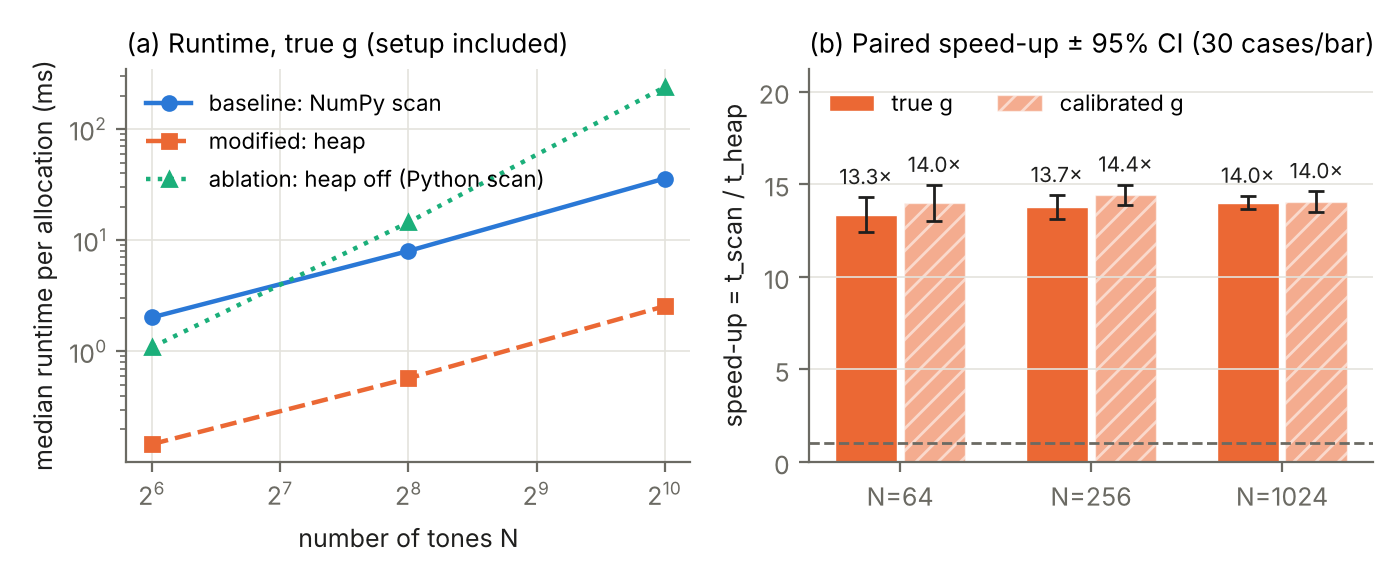
\includegraphics[width=0.62\linewidth]{../results/final/fig2_main_comparison.png}\hfill
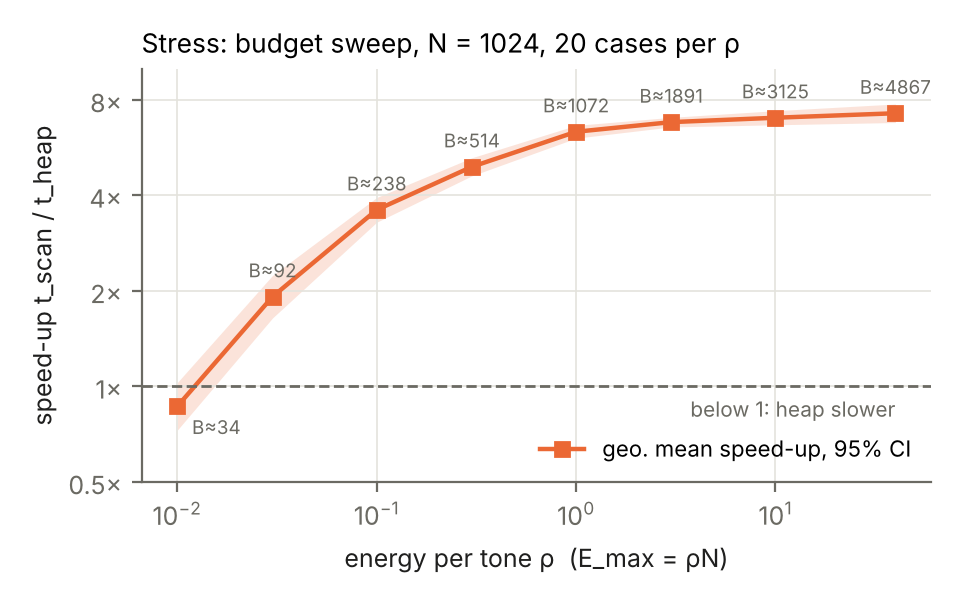
\includegraphics[width=0.37\linewidth]{../results/final/fig4_stress_budget.png}
\caption{Left: overall comparison (runtime and paired speed-up). Right: stress/failure case. With a tiny budget the
heap is no faster ($\rho=0.01$: $0.87\times$, CI $[0.73,1.03]$, about 34 bits in total). Generated by
\texttt{run\_experiments.py} from \texttt{results/final/*.csv}.}
\label{fig:main}
\end{figure}
\vspace{-6pt}

\textbf{Correctness of the change.} The allocations were \emph{identical} (bits, energy and remaining budget compared exactly) in
every one of the 1186 runs, including the flat-channel tie stress. \textbf{Speed.} The heap is about 7$\times$ faster at
$N=64$--$1024$, with tight CIs, and $12.0\times$ [11.4, 12.7] at $N=4096$ (Fig.~\ref{fig:scaling}).
\textbf{The hypothesis is only partly supported.} Between $N=64$ and $1024$ the speed-up is roughly flat, not
growing. NumPy's vectorised \texttt{argmin} costs about 2\,\textmu s per call whatever the size up to $N\approx1000$, because call overhead
dominates (Fig.~\ref{fig:scaling}). So in practice the measured baseline is not yet ``$\Theta(N)$ per step''. The growth
predicted by the asymptotic analysis appears only at $N=4096$. \textbf{The ablation} isolates the data structure. With
identical Python code, heap versus linear scan gives 9.6$\times$, 30$\times$ and 99$\times$ for $N=64,256,1024$, the textbook
$O(N)$-versus-$O(\log N)$ separation. Most of the baseline's gap to this is hidden by vectorisation, not removed.
\textbf{Failure case.} With $\rho=0.01$ the 0.09\,ms heap build is not repaid by about 34 increments, and the heap is no faster
(point estimate slower, CI includes 1). The crossover lies between $\rho=0.01$ and $0.03$ for $N=1024$. A practical
implementation could choose the method from the expected $B/N$.
\textbf{Model validity, not code correctness.} When bits are planned on $\hat g$ from 20 pilots, the true energy exceeded
$E_{\max}$ in 30/30 cases (mean $+8.9\%$, 95\% CI $[7.4,10.4]$, maximum $+18\%$). With 4 pilots the overspend was $+65\%$, and with 100 pilots $+1.5\%$
(Fig.~\ref{fig:cal}). Noise inflates $|\hat h|^2$ on average, and the greedy rule preferentially loads the tones whose
$g$ was over-estimated. Both methods are affected identically, because the change cannot fix bad inputs.
\textbf{Limitations.} The data are synthetic, the gap model is approximate, tones are independent, timing comes from a
single shared cloud machine, and only the greedy core is reproduced. The heap's advantage depends on Python and NumPy
implementation details, not only on asymptotics.

\section{Reproduction}
Repository: \url{\repo}, submitted tag \texttt{v1.0-submission} (the full commit hash is given in the
submission form). These results were produced at commit \texttt{3758433}, recorded in
\texttt{results/final/environment.json}. Commands: \texttt{python -m pip install -r requirements.txt};
\texttt{python -m pytest} (348 checks, about 1\,s); \texttt{python run\_experiments.py --config configs/smoke.json}
(about 2\,s); \texttt{python run\_experiments.py --config configs/final.json} (about 2\,min); add \texttt{--figures-only} to redraw the figures
from the saved CSVs. Tables and figures in this report come from \texttt{results/final/summary.csv} and
\texttt{fig*.png}.

\textbf{Contribution and assistance statement.} This is an individual project. The code, tests, experiments and this
report were developed with substantial help from a generative-AI assistant (Claude, Anthropic), used under the
module's AI policy. I chose the track, reviewed and ran all code, and can explain every assessed function and
result. No external code or datasets were used. The paper is cited but not redistributed.

\begin{thebibliography}{9}\small
\bibitem{campello} J.~Campello, ``Practical bit loading for DMT,'' in \emph{Proc.\ IEEE ICC}, vol.~2, 1999,
pp.~801--805. doi:10.1109/ICC.1999.765384.
\bibitem{clrs} T.~H.~Cormen, C.~E.~Leiserson, R.~L.~Rivest, C.~Stein, \emph{Introduction to Algorithms},
3rd~ed., MIT Press, 2009, ch.~6 (heaps and priority queues).
\bibitem{guide} D.~Ramsook, ``Final-project mathematical guide, Track D,'' EEP55C36 course material, TCD, 2026.
\end{thebibliography}

\clearpage
\appendix
\section*{Appendix: additional figures (generated by \texttt{run\_experiments.py})}
\begin{figure}[!t]\centering
\begin{subfigure}{0.56\linewidth}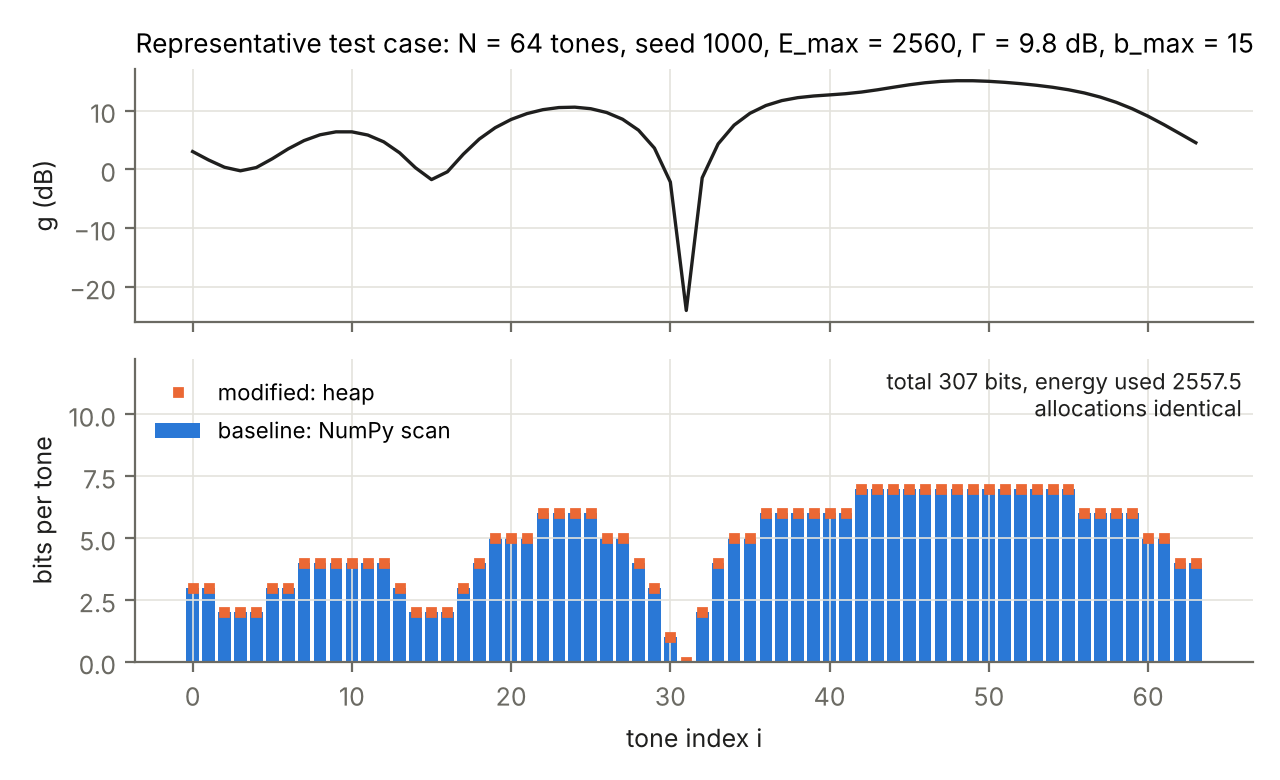
\includegraphics[width=\linewidth]{../results/final/fig1_example.png}
\caption{Representative test case: gain and identical allocations.}\end{subfigure}\hfill
\begin{subfigure}{0.42\linewidth}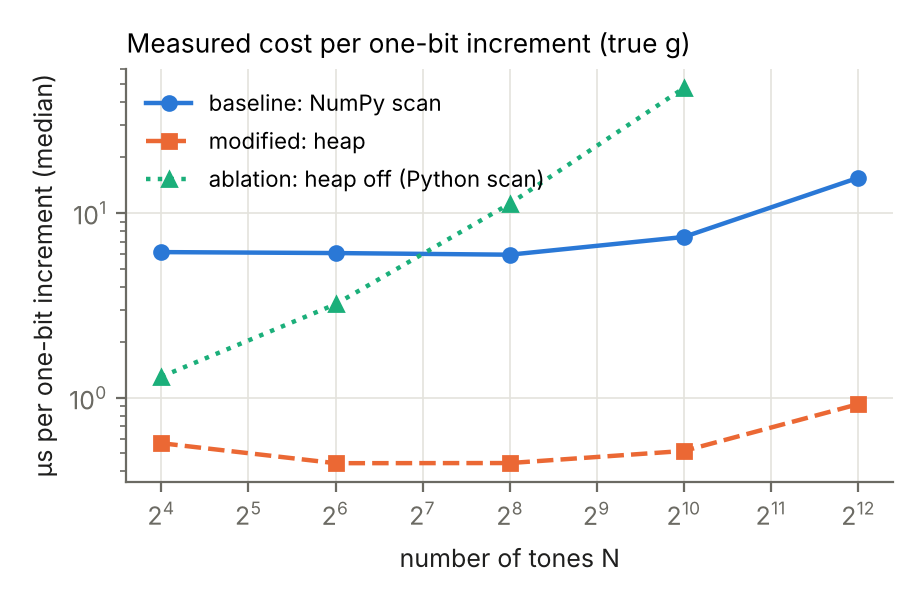
\includegraphics[width=\linewidth]{../results/final/fig3_scaling.png}
\caption{Cost per increment versus $N$.}\label{fig:scaling}\end{subfigure}\\[4pt]
\begin{subfigure}{0.45\linewidth}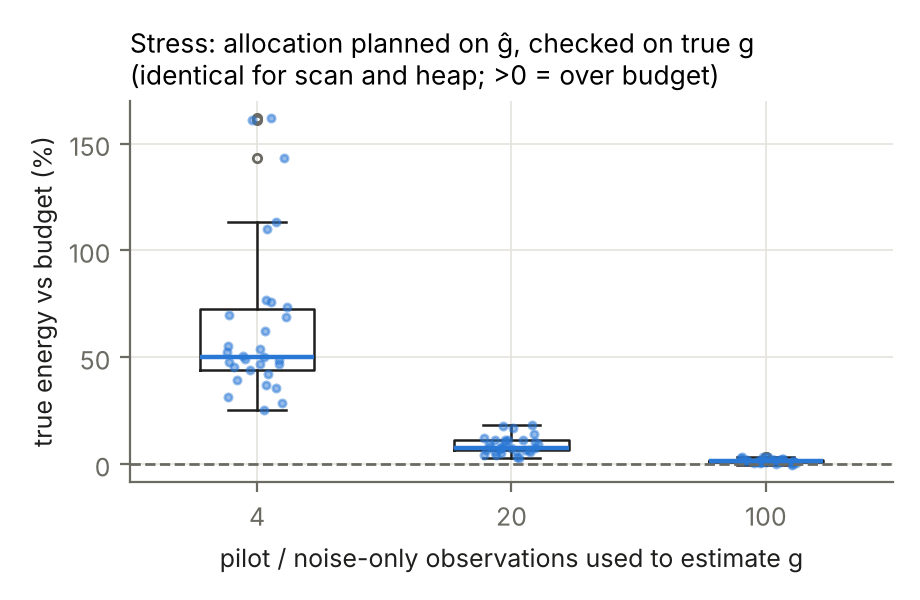
\includegraphics[width=\linewidth]{../results/final/fig5_stress_calibration.png}
\caption{Overspend of true energy when planning on $\hat g$.}\label{fig:cal}\end{subfigure}
\caption{Supporting figures.}
\end{figure}
\end{document}
